\documentclass[12pt, a4paper]{article}
\usepackage{amsmath, amsthm, amssymb, bm, color, framed, graphicx, hyperref, mathrsfs, subfigure}
\usepackage{appendix, dirtree, enumerate, float, ulem}
\usepackage{hyperref}
\usepackage{listings}
\usepackage{fancyhdr}
\usepackage{practise}
\usepackage{caption}
\usepackage{float}
\usepackage{tikz,mathpazo}
\usetikzlibrary{shapes.geometric, arrows}
\usepackage{flowchart}

\def\Name{PB20020586 叶子昂\\
		}
\def\Session{Spring 2023}
\def\LabContent{流水线 CPU 设计}

\title{\textbf{程序设计进阶与实践} \\
        设计报告}
\author{\Name \\
    
\includegraphics[width = 0.3 \textwidth]{logo.png}}
\linespread{1.5}

\titleformat{\section}[frame]
    {\Large\bfseries}
    {\thesection.}{0.5em}{}
\geometry{a4paper, centering, scale=0.8}
\graphicspath{ {./figs/} }

\lstset{style = mystyle, escapeinside=`'}


\begin{document}
\maketitle
\pagestyle{fancy}
\setlength{\headheight}{20pt}
\setlength{\headsep}{10pt}
\fancyhead[L]{\small{程序设计进阶与实践--\Session}}
\fancyhead[R]{\small{设计报告}}
\fancyfoot[C]{\small{$\thepage$}}
\newpage
\tableofcontents
\newpage

\section{需求分析}

\section{概要设计}

\section{详细设计介绍与系统设计}
我们的程序采用 Spring Boot 框架, JDBC 采用 MyBatis 管理,数据库使用 MySQL,前端使用 vue 构建,总体
使用持久层-业务层-控制层-前端的架构,下面分别介绍各个模块的设计。
\subsection{持久层}
持久层采用 MyBatis 管理,使用 Mapper.xml 文件进行数据库操作,使用 Dao 接口进行调用,针对每一个表,我们
都设计了一个 Dao 接口和一个 Mapper.xml(./resources/Mapper) 文件同时有相应的 entity 进行数据封装如下:
\begin{figure}[H]
  \centering
  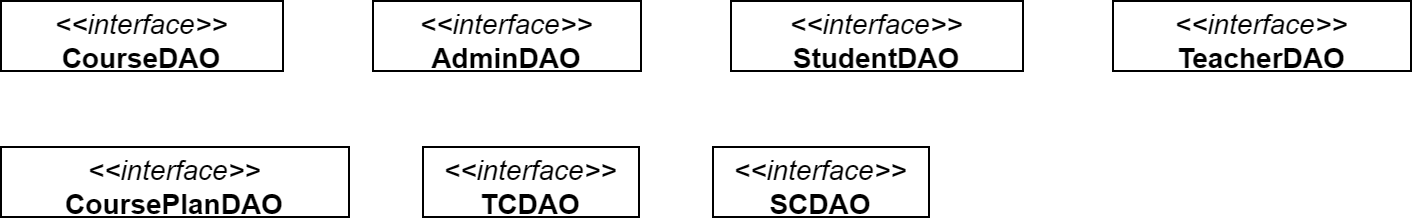
\includegraphics[width = 0.8 \textwidth]{MapperInterface.png}
  \caption{Dao 接口}
\end{figure}
\begin{figure}[H]
  \centering
  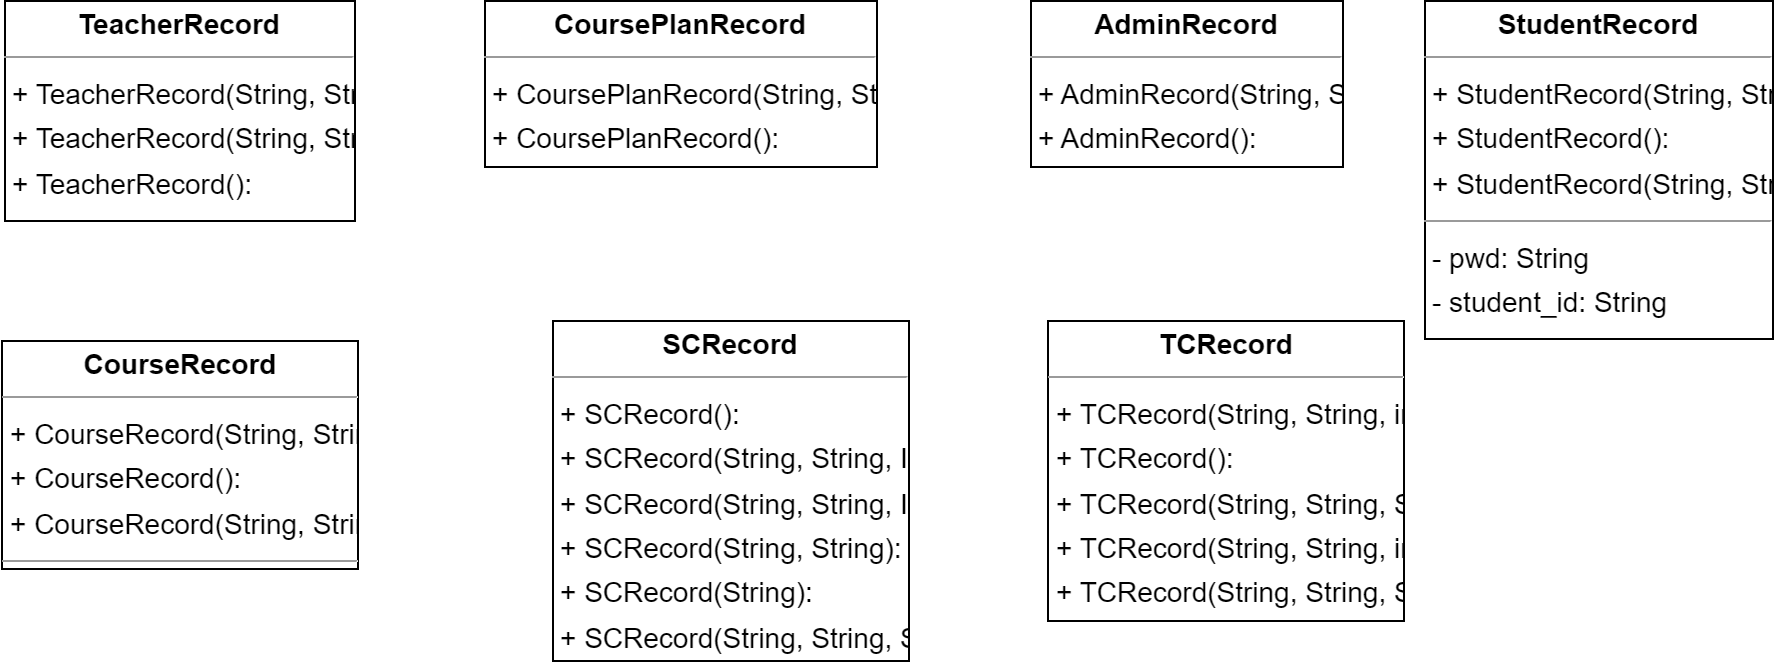
\includegraphics[width = 0.8 \textwidth]{entity.png}
  \caption{数据库实体}
\end{figure}

下面以 TeacherMapper 为例,介绍持久层接口和 Mapper.xml 文件的设计。TeacherDao 接口中定义了
如下的方法(功能见注释):
\begin{figure}[H]
  \centering
  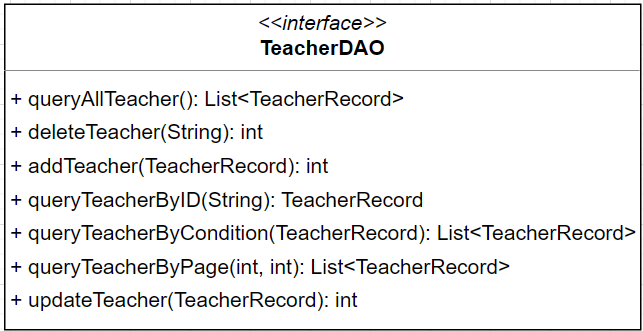
\includegraphics[width = 0.6 \textwidth]{TeacherDao.png}
  \caption{TeacherDao 接口}
\end{figure}
\begin{lstlisting}[language = Java]
@Mapper //`MyBatis 的注解,表示这是一个 Mapper 接口,会自动将其与 Mapper.xml 文件关联'
@Repository(value = "TeacherDAO")
public interface TeacherDAO {
		// `查询所有教师'
		List<TeacherRecord> queryAllTeacher();
		// `分页查询教师'
		public List<TeacherRecord> queryTeacherByPage(@Param("page") int page, @Param("size") int size);
		// `查询指定教师的 ID'
		public TeacherRecord queryTeacherByID(@Param("teacher_id") String ID);
		// `更新教师信息'
		public int updateTeacher(TeacherRecord record);
		// `删除教师'
		public int deleteTeacher(@Param("teacher_id") String ID);
		// `添加教师'
		public int addTeacher(TeacherRecord record);
		// `根据条件查询教师'
		List<TeacherRecord> queryTeacherByCondition(TeacherRecord temp);
	}
\end{lstlisting}
Mapper.xml 文件中定义了如下的 SQL 语句与之对应:
\begin{lstlisting}[language = Java]
    <select id="queryAllTeacher" resultType="com.cy.studentsel.entity.TeacherRecord">
        select * from teacher
    </select>
    <select id="queryTeacherByPage" parameterType="int" resultType="TeacherRecord">
        select * from teacher limit #{page}, #{size}
    </select>
    <select id="queryTeacherByID" resultType="TeacherRecord" parameterType="String">
        select * from teacher where teacher.teacher_id = #{teacher_id}
    </select>
    <select id="queryTeacherByCondition" resultType="TeacherRecord">
        select teacher_id, teacher_name, sex, age
        from teacher
        where
		// `如果 teacher\_id 不为空, 动态拼接 SQL 语句'
        <if test="teacher_id != null and teacher_id != ''">
            teacher_id like concat('%', #{teacher_id}, '%') and // `模糊查询'
        </if>
        <if test="teacher_name != null and teacher_name != ''">
            teacher_name like concat('%', #{teacher_name}, '%') and
        </if>
        <if test="sex != null and sex != ''">
            sex = #{sex} and
        </if>
        <if test="age != null and age != -1">
            age = #{age} and
        </if>
        true
    </select>
    <update id="updateTeacher" parameterType="TeacherRecord">
        update teacher
        <set>
		// `如果 teacher\_name 不为空, 动态拼接 SQL 语句'
            <if test="teacher_name != null and teacher_name != ''"> 
                teacher_name = #{teacher_name},
            </if>
            <if test="sex != null and sex != ''">
                sex = #{sex},
            </if>
            <if test="age != null and age != -1">
                age = #{age},
            </if>
            <if test="pwd != null and pwd != ''">
                pwd = #{pwd},
            </if>
            teacher_id = #{teacher_id}
        </set>
        <where>
            teacher_id = #{teacher_id}
        </where>
    </update>
    <delete id="deleteTeacher" parameterType="String">
        call deleteTeacher(#{teacher_id})
    </delete>
    <insert id="addTeacher" parameterType="TeacherRecord">
        insert into teacher values (#{teacher_id}, #{teacher_name}, #{sex}, #{age}, #{pwd})
    </insert>
\end{lstlisting}

其中 deleteTeacher 为保证数据一致性设计为一个存储过程(因为删去教师需要同时删去教师的授课信息):
\begin{lstlisting}[language = Java]
	// `删除教师记录事务'
	drop procedure if exists deleteTeacher;
	delimiter //
	create procedure deleteTeacher(in teacher_id varchar(20))
	begin
		delete from TC where tc.teacher_id=teacher_id;
		delete from Teacher where teacher.teacher_id=teacher_id;
	end //
	delimiter ;
\end{lstlisting}
对于删去学生和课程的操作也是类似的。

\subsection{业务层}
\subsubsection{控制层主要功能类}
业务层主要负责对持久层的调用以及包装来定义业务逻辑以供控制层调用,是的控制层不需要关心具体的
数据库实现使得将控制层与持久层解耦合。我们定义如下形式的业务层接口:
\begin{figure}[H]
  \centering
  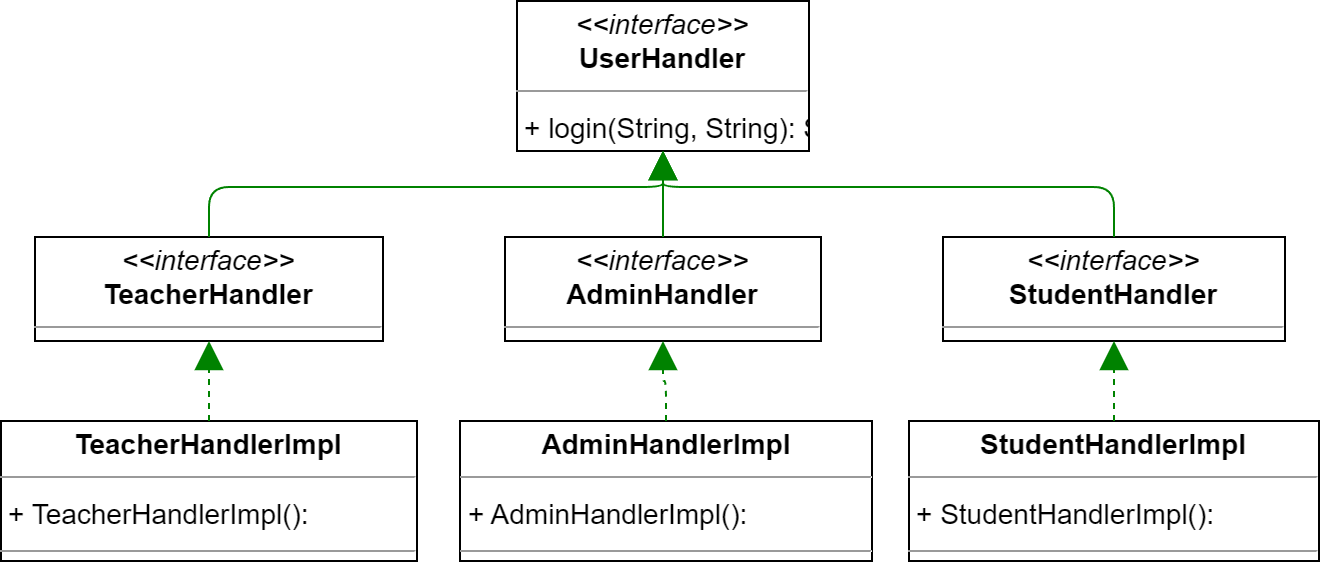
\includegraphics[width = 0.8 \textwidth]{ServiceInterface.png}
  \caption{Handler 接口}
\end{figure}
下面以 TeacherHandler 为例,介绍业务层的设计。TeacherHandler 接口实现了 UserHandler 接口
(其中的 login 是每个 Handler 都需要提供的),TeacherHandler 接口中定义了如下的方法:
\begin{figure}[H]
  \centering
  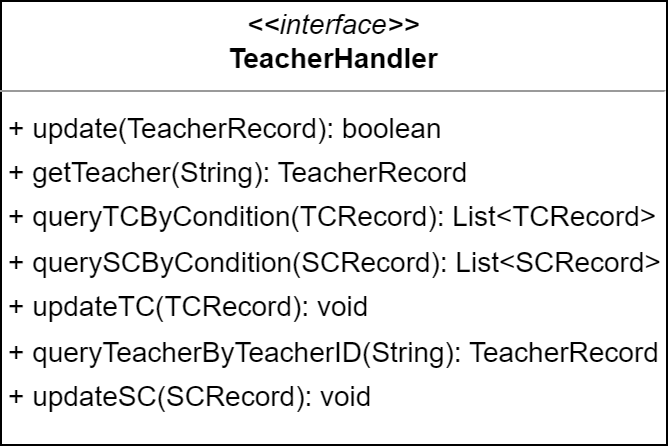
\includegraphics[width = 0.6 \textwidth]{TeacherHandler.png}
  \caption{TeacherHandler 接口}
\end{figure}
TeacherHandlerImpl 类中实现了 TeacherHandler 接口中的方法如下:
\begin{lstlisting}[language = Java]
	@Service // `标注为 Spring 的 Service 层'
	public class TeacherHandlerImpl implements TeacherHandler {
		@Resource	// `自动注入 TeacherDAO 对象'
		private TeacherDAO teacherDao;
		@Resource	// `自动注入 SCDAO 对象'
		private SCDAO scDao;
		@Resource	// `自动注入 TCDAO 对象'
		private TCDAO tcDao;
	
		@Override
		public String login(String ID, String pwd) {
			TeacherRecord teacherRecord = teacherDao.queryTeacherByID(ID);
			if (teacherRecord == null) {
				throw new UserNameNoFoundException("`教师工号不存在'");
			}
			if (!Objects.equals(teacherRecord.getPwd(), pwd)){
				throw new PasswordNoMatchException("`密码错误'");
			}
			return "`登录成功'";
		}
	
		// `查询教师信息'
		@Override
		public List<TCRecord> queryTCByCondition(TCRecord record) {
			return tcDao.queryTCByCondition(record);
		}
		// `通过 ID 查询教师信息'
		@Override
		public TeacherRecord getTeacher(String ID) {
			return teacherDao.queryTeacherByID(ID);
		}
	 	// `更新教师信息'
		@Override
		public boolean update(TeacherRecord teacherRecord) {
			teacherDao.updateTeacher(teacherRecord);
			return true;
		}
		// `查询选本教师课的所有选课记录'
		@Override
		public List<SCRecord> querySCByCondition(SCRecord record) {
			return scDao.querySCByCondition(record);
		}
		// `更新授课信息'
		@Override
		public void updateTC(TCRecord record) {
			tcDao.updateTC(record);
		}
		// `更新选课信息(评分)'
		@Override
		public void updateSC(SCRecord record) {
			scDao.updateSC(record);
		}
	
	}
\end{lstlisting}
其中 TeacherHandlerImpl 类中的 TeacherDAO、SCDAO、TCDAO 为持久层接口。
\subsubsection{业务层异常}
业务层执行部分持久层操作前,需要对传入的参数进行检查,如果参数不合法,需要抛出异常。业务层的异常自定义
为 RuntimeException 的子类,如下:
\begin{figure}[H]
  \centering
  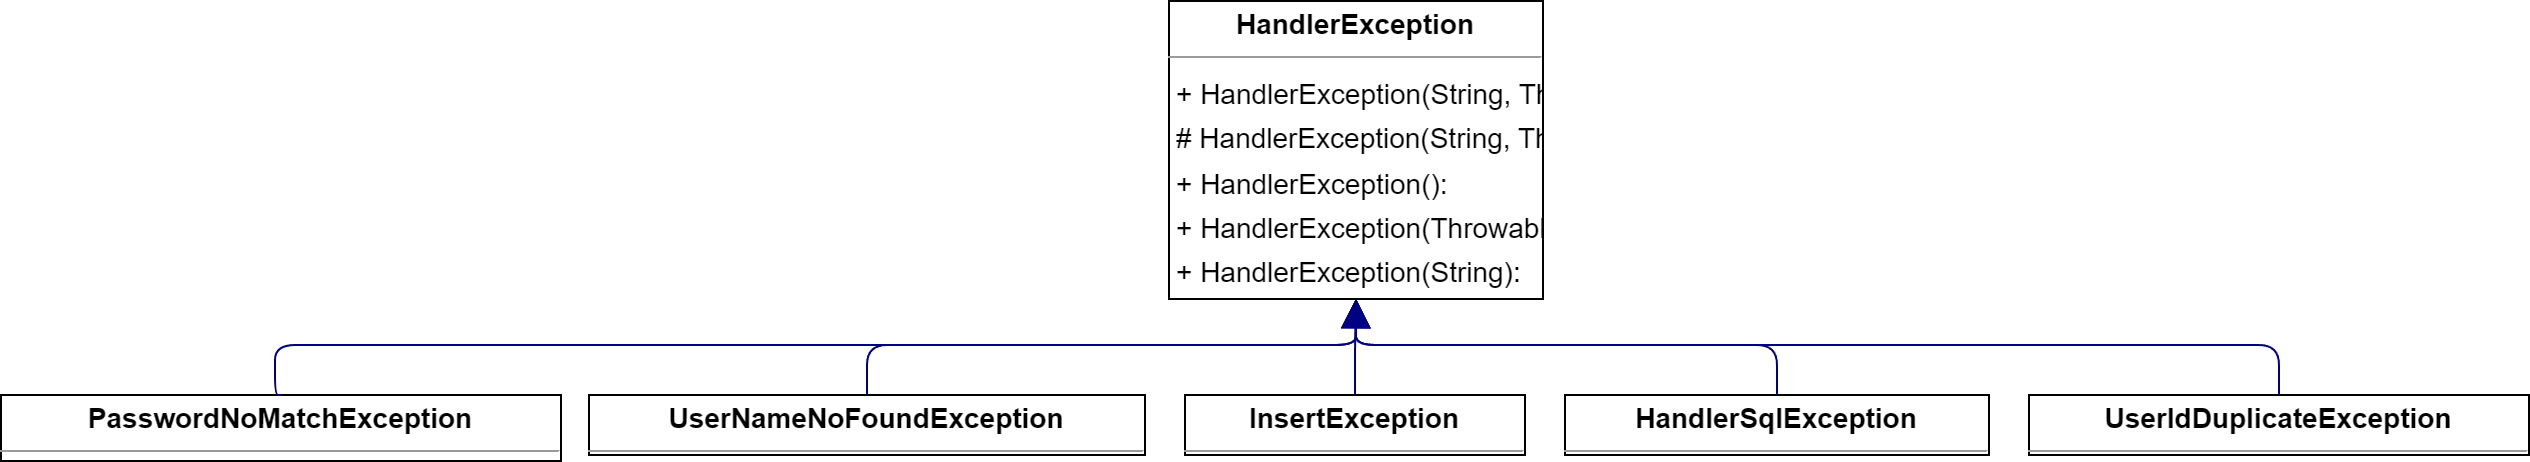
\includegraphics[width = 0.9 \textwidth]{HandlerException.png}
  \caption{业务层异常}
\end{figure}

\subsection{控制层}
\subsubsection{控制层主要功能类}
控制层主要负责接收用户的请求,直接面向前端提供方法,整合业务层的方法。我们定义如下控制层类:
\begin{figure}[H]
  \centering
  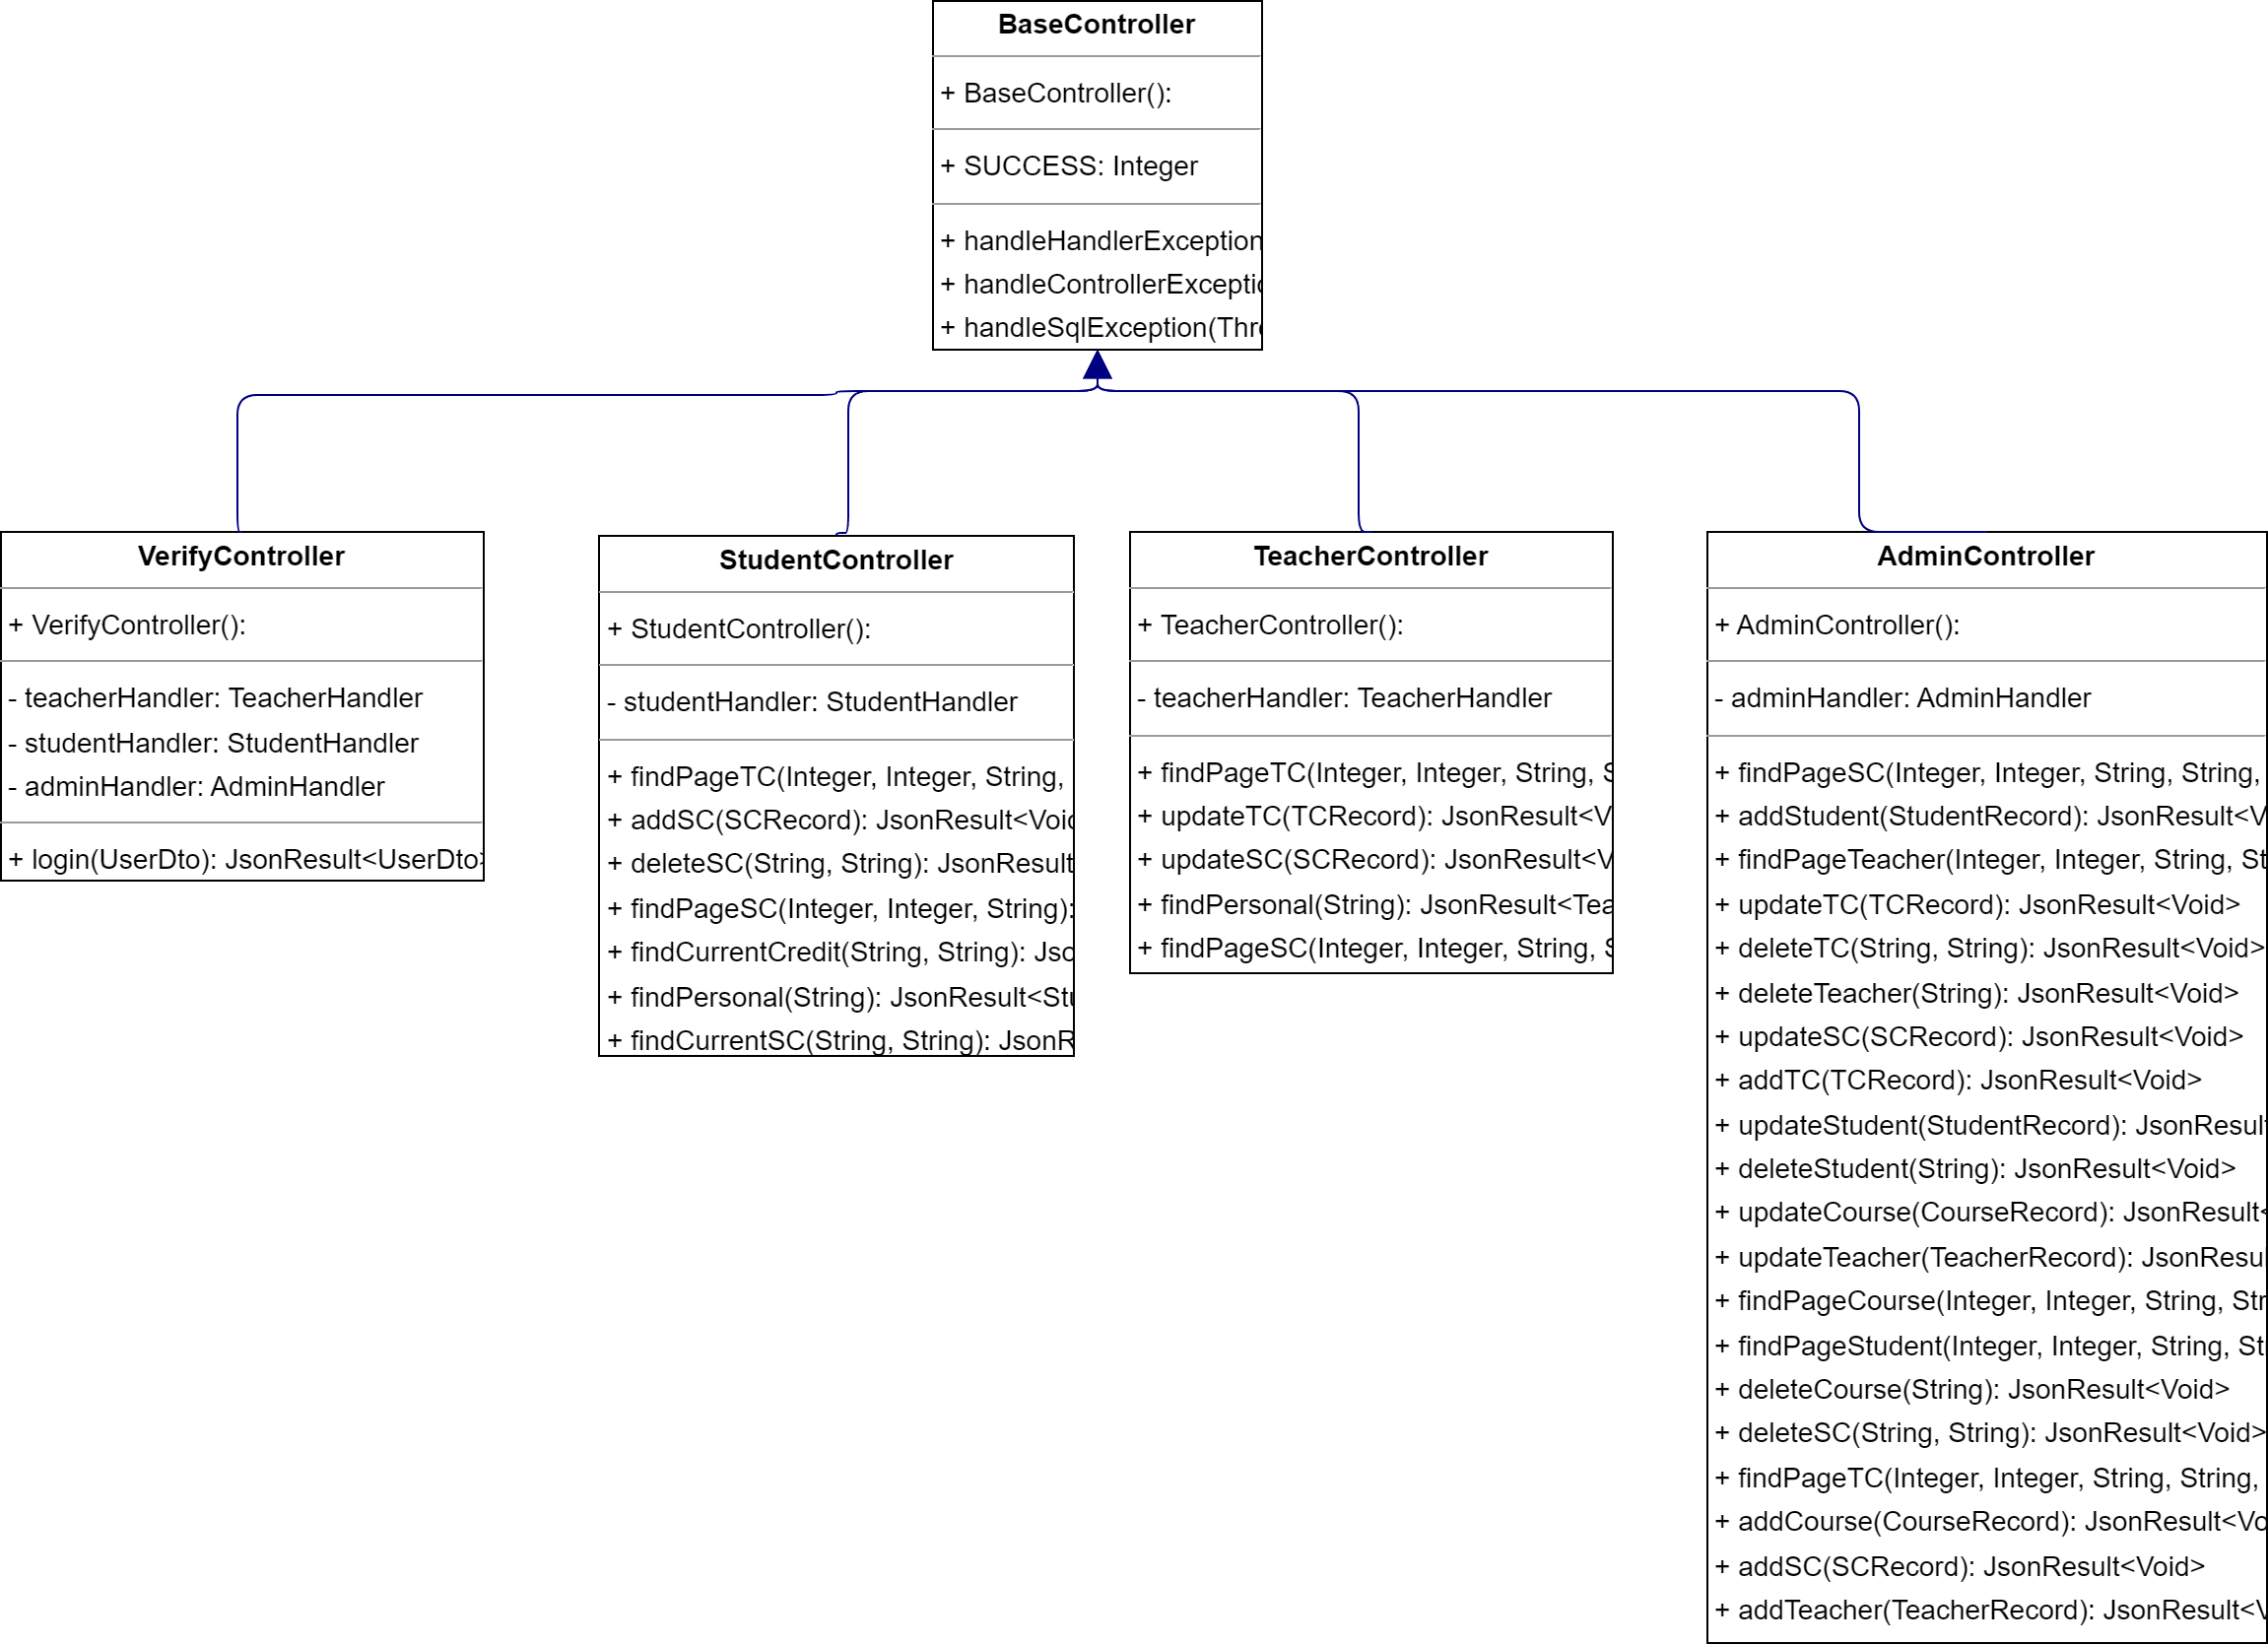
\includegraphics[width = 0.9 \textwidth]{Controller.png}
  \caption{控制层类}
\end{figure}

其中:
\begin{itemize}
  \item BaseController 类:提供所有控制层类的基类,提供统一的全局异常处理机制
  \item VerifyController 类:提供针对所有用户的统一登录验证
  \item AdminController 类:提供管理员前端界面所需的所有方法
  \item TeacherController 类:提供教师前端界面所需的所有方法
  \item StudentController 类:提供学生前端界面所需的所有方法
\end{itemize}

以 TeacherController 类为例,介绍控制层的设计。TeacherController 类中定义了如下方法:
\begin{figure}[H]
  \centering
  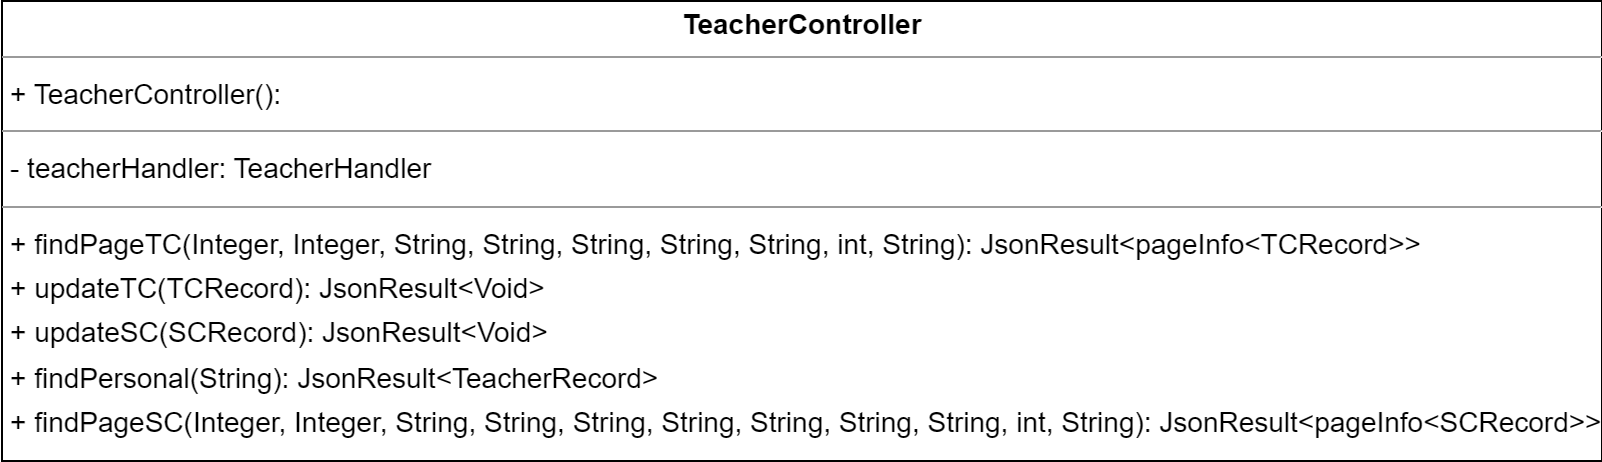
\includegraphics[width = 0.9 \textwidth]{TeacherController.png}
  \caption{TeacherController 类}
\end{figure}
\begin{itemize}
  \item findPageTC 方法:处理教师分页查询授课信息的请求
  \item updateTC 方法:处理教师更新授课信息的请求
  \item updateSC 方法:处理教师更新学生选课信息(评分)的请求
  \item findPersonal 方法:处理登录时查询个人信息
  \item findPageSC 方法:处理教师分页查询选自己课学生信息的请求
\end{itemize}
\begin{lstlisting}[language=Java]
	@RestController`// 标注为 Spring 的 Controller 层,自动将返回值转换为 JSON 对象'
	@RequestMapping("api/teacher")
	public class TeacherController extends BaseController{
	@Resource
	private TeacherHandler teacherHandler;

	/**
	* get teacher personal information
	*/
	@GetMapping("/personal")
	@ResponseBody
	public JsonResult<TeacherRecord> findPersonal(@RequestParam String teacher_id) {
		JsonResult<TeacherRecord> jsonResult = new JsonResult<>();
		TeacherRecord record = teacherHandler.queryTeacherByTeacherID(teacher_id);
		jsonResult.setData(record);
		jsonResult.setStatus(SUCCESS);
		jsonResult.setMsg("`查询成功'");
		return jsonResult;
	}

	/**
		* All the student who choose the course in page range
		*/
	@GetMapping("/page/sc")
	@ResponseBody
	public JsonResult<pageInfo<SCRecord>> findPageSC(@RequestParam Integer page,
													@RequestParam Integer pageSize,
													@RequestParam String student_id,
													@RequestParam String student_name,
													@RequestParam String course_id,
													@RequestParam String course_name,
													@RequestParam String teacher_id,
													@RequestParam String teacher_name,
													@RequestParam String type,
													@RequestParam int credit,
													@RequestParam String place) {
		JsonResult<pageInfo<SCRecord>> jsonResult = new JsonResult<>();
		pageInfo<SCRecord> pageInfo = new pageInfo<>();
		SCRecord record = new SCRecord(student_id, course_id, teacher_id, 
				student_name, course_name, teacher_name, type, credit, place);
		List<SCRecord> list = teacherHandler.querySCByCondition(record);
		int pageStart = (page - 1) * pageSize;
		int limit = pageSize;
		pageInfo.list = list.subList(pageStart, min(pageStart + limit, list.size()));
		pageInfo.total = list.size();
		jsonResult.setData(pageInfo);
		jsonResult.setStatus(SUCCESS);
		jsonResult.setMsg("`查询成功'");
		return jsonResult;
	}
	.......
	`部分方法实现与上面方法类似且相对较长,不再赘述见源码'

	}
\end{lstlisting}

\subsubsection{登录鉴权与操作鉴权}
登录鉴权是指用户在访问系统资源时,系统对用户进行身份验证的过程。本系统中,用户登录后,系统会为用户生成一个 token
(限制有效时间为 15 分钟)返回给前端,前端将得到的 token 存储在本地,每次请求时将 token 放在请求头中,后端会对 token 进行
不同权限的操作进行鉴权,如果 token 过期或者 token 不合法,后端会返回错误信息,前端会跳转到登录界面。登录鉴权的实现
通过如下类:
\begin{figure}[H]
  \centering
  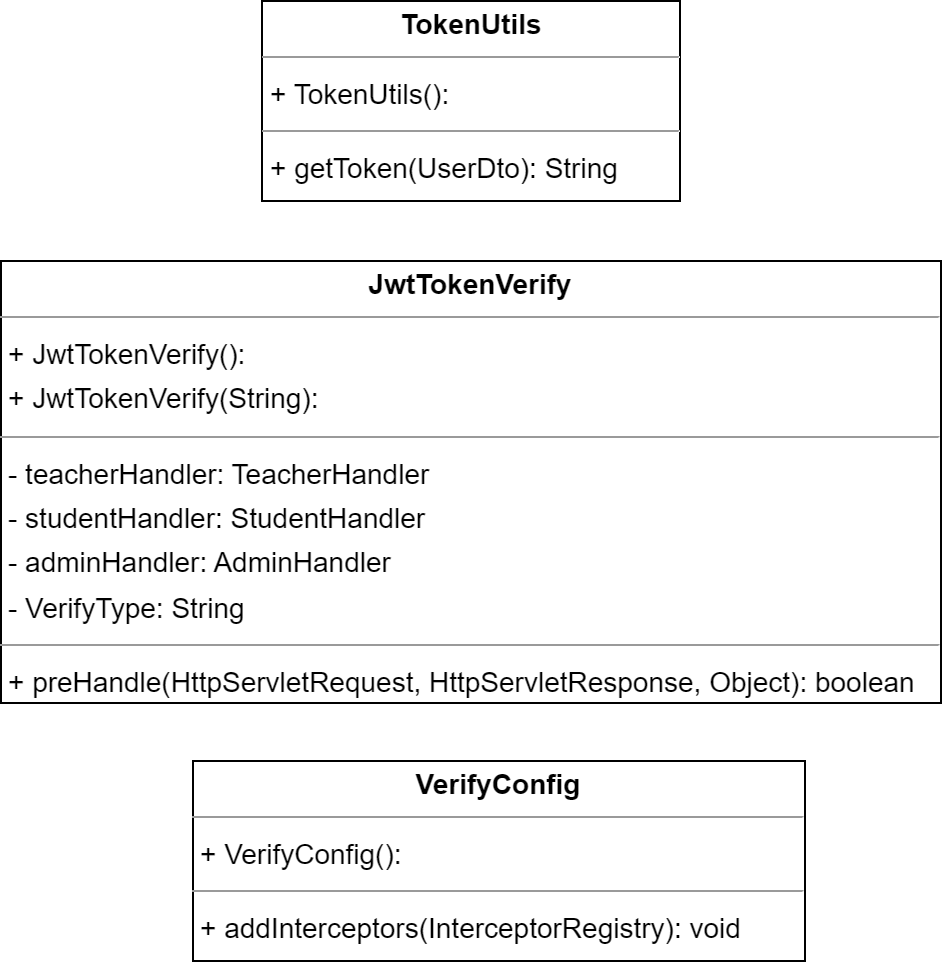
\includegraphics[width = 0.5 \textwidth]{loginVerify.png}
  \caption{登录鉴权}
\end{figure}
其中:
\begin{itemize}
  \item TokenUtil 类:提供依据用户名,用户类型,用户签名生成 token 的方法(使用 HMAC256 算法)
  \item JwtTokenVerify 类:提供基于不同用户类型的 token 验证方法
  \item VerifyConfig 类:提供 token 验证的拦截器配置
\end{itemize}
依次实现如下:\\
\textbf{TokenUtil.java}
\begin{lstlisting}[language=Java]
	/**
	* `生成 Token'
	*/
	public static String getToken(UserDto userDto) {
			String token="";
			token= JWT.create().withClaim("username", userDto.getUsername())// `保存用户信息'
				.withClaim("userType", userDto.getUserType())// `保存用户信息'
				.withExpiresAt(DateUtil.offsetMinute(new Date(), 15))// `设置过期时间为 15 分钟'
				.sign(Algorithm.HMAC256(userDto.getPassword()));// `以 password 作为 token 的密钥'
			return token;
		}
\end{lstlisting}
\textbf{JwtTokenVerify.java}
\begin{lstlisting}[language=Java]
	@Override
	public boolean preHandle(HttpServletRequest request, HttpServletResponse response, Object handler) {
			String token = request.getHeader("token");
			if (!(handler instanceof HandlerMethod))
					return true;
			if (token == null || token.equals("")) {
					throw new NoTokenException("`未登录'");
			}

			String username;
			String userType;
			String password;
			try {
					username = JWT.decode(token).getClaim("username").asString();
					userType = JWT.decode(token).getClaim("userType").asString();
					// if the token is not for the requested user type, then throw exception
					if (!userType.equals(VerifyType)) {
							throw new VerifyTokenFailException("`token 验证失败'");
					}
					// get the password from database
					switch (userType) {
							case "admin" -> {
									AdminRecord adminRecord = adminHandler.getAdmin(username);
									password = adminRecord.getPwd();
							}
							case "teacher" -> {
									TeacherRecord teacherRecord = teacherHandler.getTeacher(username);
									password = teacherRecord.getPwd();
							}
							case "student" -> {
									StudentRecord studentRecord = studentHandler.getStudent(username);
									password = studentRecord.getPwd();
							}
							default -> throw new VerifyTokenFailException("`token 验证失败'");
					}
					// verify the token
					JWTVerifier jwtVerifier = JWT.require(Algorithm.HMAC256(password)).build();
					jwtVerifier.verify(token);
			} catch (Exception e) {
					throw new VerifyTokenFailException("`token 验证失败'");
			}							
			return true;
	
\end{lstlisting}
\textbf{VerifyConfig.java}
\begin{lstlisting}[language=Java]
	/**
	*  `拦截请求,验证 token,登录请求不必验证'
	* @param registry
	*/
 @Override
 public void addInterceptors(InterceptorRegistry registry) {
		 // if /api/admin is requested, then verify the token with admin role
		 registry.addInterceptor(jwtTokenVerifyAdmin())
						 .addPathPatterns("/api/admin/**")
						 .excludePathPatterns("api/verify");
		 // if /api/teacher is requested, then verify the token with teacher role
		 registry.addInterceptor(jwtTokenVerifyTeacher())
						 .addPathPatterns("/api/teacher/**")
						 .excludePathPatterns("/api/verify");
		 // if /api/student is requested, then verify the token with student role
		 registry.addInterceptor(jwtTokenVerifyStudent())
						 .addPathPatterns("/api/student/**")
						 .excludePathPatterns("/api/verify");
 }
\end{lstlisting}

\subsubsection{控制层异常处理}
控制层在请求业务层操作前,需要对传入的参数进行一定的检查(包括权限检查,登录请求类型检查),当登录参数不合法以及
请求的权限不足时,需要抛出异常。控制层的异常自定义为 RuntimeException 的子类,如下:
\begin{figure}[H]
  \centering
  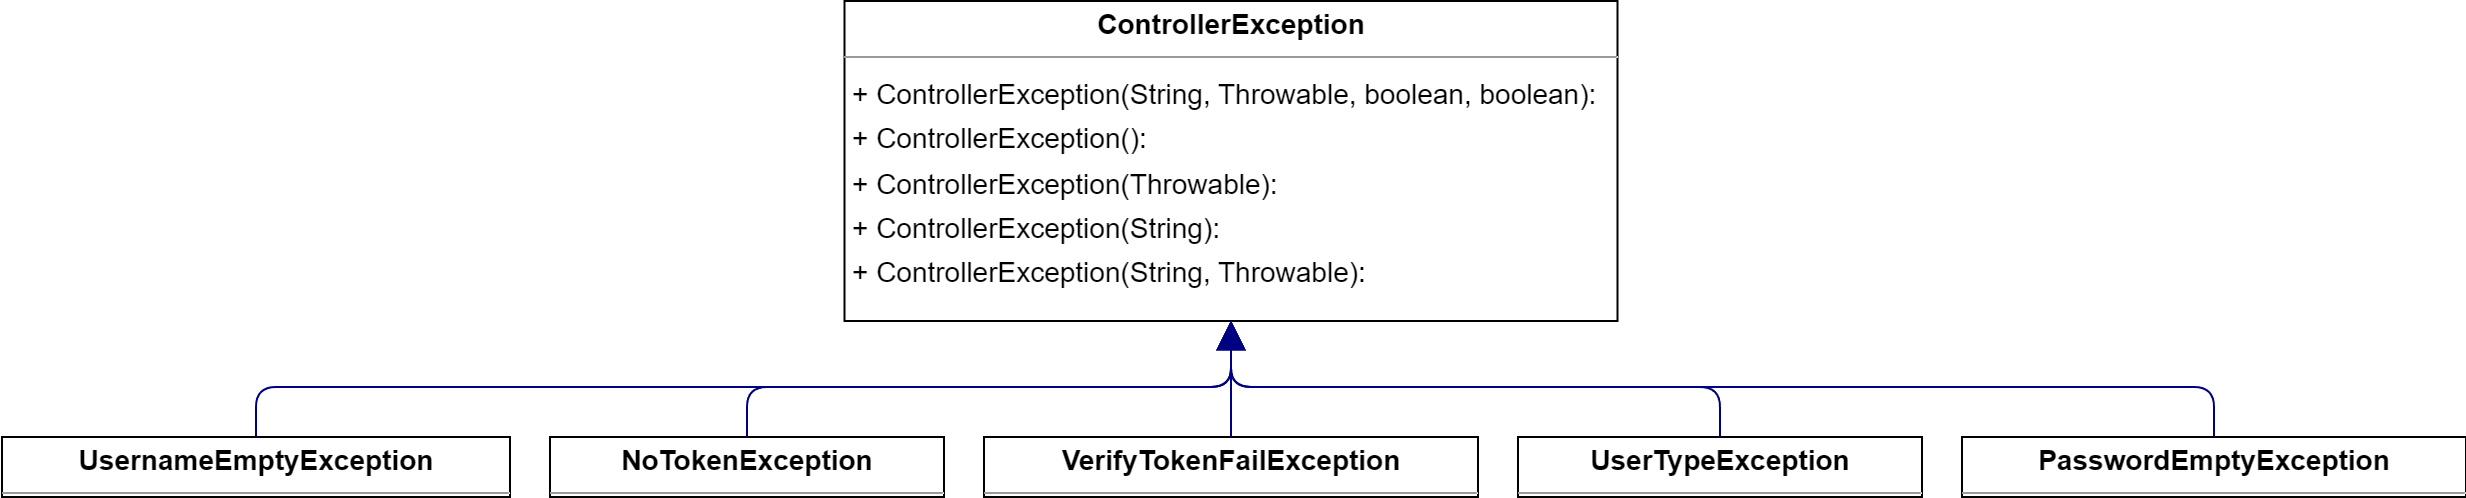
\includegraphics[width = 0.9 \textwidth]{ControllerException.png}
  \caption{控制层异常}
\end{figure}

\subsection{全局异常处理机制}
在项目中我们在业务层和控制层抛出自定义异常,数据库在操作时也可能可能由于服务器宕机等各种原因抛出异常,
在将问题传递给前端前需要将异常信息进行处理避免造成程序崩溃。
我们选择在控制层统一捕获各类异常进行处理。
异常的处理在 BaseController 类中实现,所有的控制层 Controller 都继承自 BaseController,拥有统一的
异常处理机制。\\
\textbf{业务层异常处理}
\begin{lstlisting}[language=Java]
	/**
	* Handle the exception thrown by the service layer
	* @param e
	* @return
	*/
 @ExceptionHandler(HandlerException.class)// `Java 注释,自动捕获所有业务层异常'
 @ResponseBody
 public JsonResult<Void> handleHandlerException(Throwable e) {
		 JsonResult<Void> jsonResult = new JsonResult<>();
		 switch (e.getClass().getSimpleName()) {
				 case "UserNameNoFoundException" -> {
						 jsonResult.setStatus(1000);
						 jsonResult.setMsg(e.getMessage());
				 }
				 case "PasswordNoMatchException" -> {
						 jsonResult.setStatus(1001);
						 jsonResult.setMsg(e.getMessage());
				 }
				 case "UserIdDuplicateException" -> {
						 jsonResult.setStatus(1002);
						 jsonResult.setMsg(e.getMessage());
				 }
				 case "HandlerSqlException" -> {
						 jsonResult.setStatus(5000);
						 jsonResult.setMsg(e.getMessage());
				 }
				 default -> {
						 jsonResult.setStatus(5001);
						 jsonResult.setMsg("`未知错误'");
				 }
		 }
		 return jsonResult;
 }
\end{lstlisting}
\textbf{控制层异常处理}
\begin{lstlisting}[language=Java]
	/**
	* Handle the exception thrown by the controller layer
	* @param e
	* @return
	*/
 @ExceptionHandler(ControllerException.class) //`Java 注释,自动捕获所有控制层异常'
 @ResponseBody
 public JsonResult<Void> handleControllerException(Throwable e) {
		 JsonResult<Void> jsonResult = new JsonResult<>();
		 switch (e.getClass().getSimpleName()) {
				 case "UsernameEmptyException" -> {
						 jsonResult.setStatus(2000);
						 jsonResult.setMsg(e.getMessage());
				 }
				 case "PasswordEmptyException" -> {
						 jsonResult.setStatus(2001);
						 jsonResult.setMsg(e.getMessage());
				 }
				 case "UserTypeEmptyException" -> {
						 jsonResult.setStatus(2002);
						 jsonResult.setMsg(e.getMessage());
				 }
				 case "NoTokenException" -> {
						 jsonResult.setStatus(401);
						 jsonResult.setMsg("`未登录'");
				 }
				 case "VerifyTokenFailException" -> {
						 jsonResult.setStatus(401);
						 jsonResult.setMsg("`权限不足,重新登录'");
				 }
				 default -> {
						 jsonResult.setStatus(6004);
						 jsonResult.setMsg("`控制层未知错误'");
				 }
		 }
		 return jsonResult;
 }
\end{lstlisting}
\textbf{持久层异常处理}
\begin{lstlisting}[language=Java]
	/**
	* Handle the exception thrown by the mybatis
	* @param e
	* @return
	*/
 @ExceptionHandler(SQLException.class)// `Java 注释,自动捕获所有数据库操作异常'
 @ResponseBody
 public JsonResult<Void> handleSqlException(Throwable e) {
		 JsonResult<Void> jsonResult = new JsonResult<>();
		 jsonResult.setStatus(6000);
		 jsonResult.setMsg("`Sql 错误'");
		 return jsonResult;
 }
\end{lstlisting}


\subsection{前端与后端交互封装}
前端与后端交互使用 Ajax 技术(进一步使用 axios 进行封装),我们约定使用 JSON 格式传递数据,后端通过 Spring Boot
框架提供的 @ResponseBody @RequestBody 注解分别将传出传入数据转换为 JSON 格式。
包装的格式如下:
\begin{figure}[H]
  \centering
  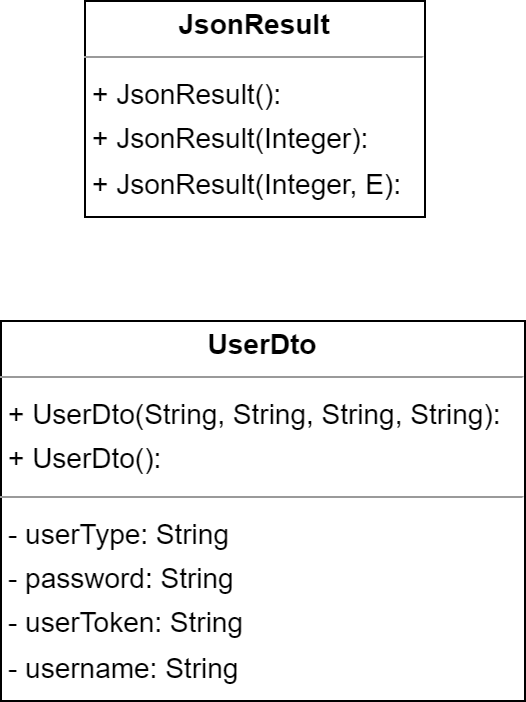
\includegraphics[width = 0.4 \textwidth]{Json.png}
  \caption{JSON 封装}
\end{figure}
其中:
\begin{itemize}
  \item JsonResult 是一个泛型类,用于封装后端传递给前端的数据,包括状态码和信息
  \item UserDto 由于封装登录时前端传递的数据,包括用户名,密码,用户类型
  \item 在持久层提到的数据库实体类用于封装从数据库中查询出的数据以及封装前端传递的数据
\end{itemize}

\subsection{第三方类引入}
为支持项目一些特殊功能,我们引入了一些第三方类库,它们分别是:
\begin{itemize}
  \item \textbf{Spring Boot 框架}:用于管理项目,提供控制反转特性的容器,托管
        项目的控制层,业务层,持久层,以及其他组件的注入。
  \item \textbf{MyBatis 框架}:用于管理数据库,提供持久层接口与 mySql 数据库的映射。
  \item \textbf{Jwt}: 用于生成 token 以及验证 token 的有效性。
  \item \textbf{hutool}: 提供方便有效的时间管理机制(设置 token 的有效时间)。

\end{itemize}

\section{调试与测试}
项目的调试与测试主要分为两个部分,前端的调试与测试,后端的调试与测试。
前端的调试通过 Postman 进行,后端的调试基于 Junit 进行单元测试。下面
举例介绍部分功能的单元测试。
\subsection{后端单元测试}
\subsubsection{数据库连接测试}
\begin{lstlisting}[language=Java]
	@SpringBootTest
	class StudentSelApplicationTests {
		@Autowired
		private DataSource DataS;
	
		@Test
		void getConnection() throws SQLException {
			System.out.println(DataS.getConnection());
		}
	}
\end{lstlisting}

\subsubsection{管理员后端业务层功能测试}
\begin{lstlisting}[language=Java]
  @SpringBootTest// `注释,自动创建 Spring Boot 容器'
  public class TestAdminHanderImpl {
      @Autowired// `注释,自动注入 AdminHandlerImpl 对象'
      private AdminHandler adminHandler;

      @Test
      public void testQueryStudentByCondition() {
          StudentRecord record = new StudentRecord("", "", "", 20, "", "");
          System.out.println(adminHandler.queryStudentByCondition(record));
      }

      @Test
      public void testUpdateStudent() {
          StudentRecord record = new StudentRecord("20160001", "", "`女'", -1, "123", "");
          adminHandler.updateStudent(record);
      }
  }
	
\end{lstlisting}

\subsubsection{学生后端业务层功能测试}
\begin{lstlisting}[language=Java]
  @SpringBootTest\\ `注释,自动创建 Spring Boot 容器'
  public class TestStudentHandlerImpl {
      @Autowired\\ `注释,自动注入 StudentHandlerImpl 对象'
      private StudentHandler studentHandler;
      @Test
      public void testlogin(){System.out.println(studentHandler.login("PB42000001","123456"));}
      @Test
      public void testgetstudent(){System.out.println(studentHandler.getStudent("PB42000001"));}
      @Test
      public void testupdate(){
          StudentRecord a=new StudentRecord("PB42000001","llf","`男'",21,"cs","123456");
          System.out.println(studentHandler.update(a));
      }
  
  
  }

\end{lstlisting}

\subsection{前端功能测试}
前端主要通过浏览器开发者模式,Postman 进行测试,主要检查点击交互时前端是否向后端发送了预期的
请求,以及后端是否返回了预期的数据。下面以登录功能为例进行测试。




\section{源程序清单与执行结果}
本项目的源代码托管在华为云 CodeArt 上, 源代码遵循如下目录结构:
\newpage

\dirtree{%
  .1 /\DTcomment{上级文件夹}.
  .2 StudentSel.
  .3 report\DTcomment{实验报告文件夹}.
  .3 SQL.
  .4 Table.Sql \DTcomment{数据库表结构文件}.
  .3 src\DTcomment{后端项目源文件}.
  .4 main.
  .5 java.
  .6 com.cy.studentsel.
  .7 Config \DTcomment{后端鉴权拦截器配置}.
  .7 controller \DTcomment{后端项目控制层}.
  .8 dto \DTcomment{后端登录数据传输对象}.
  .8 ex \DTcomment{控制层自定义异常}.
  .8 TokenVerify \DTcomment{鉴权验证器}.
  .8 BaseController.java \DTcomment{控制层基类,提供全局异常处理}.
  .8 VerifyController.java \DTcomment{控制层统一登录验证}.
  .7 DAO \DTcomment{后端项目持久层}.
  .7 entity \DTcomment{后端项目数据库实体类}.
  .7 Handler \DTcomment{后端项目业务层}.
  .8 ex \DTcomment{业务层自定义异常}.
  .8 impl \DTcomment{业务层实现}.
  .7 util \DTcomment{后端项目工具类}.
  .7 StudentSelApplication.java \DTcomment{后端项目启动}.
  .5 resources.
  .6 Mapper \DTcomment{后端项目数据库操作 xml 文件}.
  .6 application.properties \DTcomment{后端项目配置文件}.
  .4 test \DTcomment{后端项目测试文件}.
  .3 pom.xml \DTcomment{后端项目依赖}.
  .3 vue \DTcomment{前端项目文件夹}.
  .4 src \DTcomment{前端项目源文件}.
  .5 router \DTcomment{前端项目路由配置}.
  .5 views \DTcomment{前端项目页面}.
  .5 components \DTcomment{前端项目组件}.
  .5 utils \DTcomment{前端项目工具类}.
}
未标明的文件夹一般为项目自动生成框架,标出的文件夹中未注明的文件
其作用与文件名相同,不再赘述。\\
执行结果见 report 文件夹下的 result.mp4.

\section{总结}
这次课程设计,我们综合运用了课程提到的工程化开发方法,在一个具有一定规模的项目开发中我们
深刻体会到了工程项目与个人项目的区别以及规范化开发的重要性。扭转了我们平时一般先写代码
别写边想的开发习惯,在开发前我们先进行了详细的需求分析,然后进行了详细的规划设计,最后
才根据规划进行编码。

这次课程设计由我们整个小组一起完成,虽然大多数成员没有接触过前后端分离的开发,以及项目用到的
很多技术(包括 Spring Boot 框架,Mybatis 接口,Vue 前端脚手架,Jwt 鉴权),但是我们通过查阅资料,、
跟着晚上的视频根据预先的设计需求学习相应的技术,明确分工共同协作,遇到问题积极询问,互相讨论
不断迭代完善需求,最终完成了这个项目。

因为能力有限,这个项目还有很多不足之处,比如前端页面的美观程度,后端代码的优化程度,以及更多
个性化需求的实现以及代码的健壮性。但是我们会在以后的学习中不断完善这个项目,同时也会在以后的
学习中不断提高自己的能力积累高质量代码开发经验,为以后的工作打下坚实的基础。




\end{document}